\documentclass[a4paper,10pt,titlepage]{article}
% PREUMBULUM
\usepackage[utf8]{inputenc}
\usepackage[T1]{fontenc}

\usepackage{a4wide} 
\usepackage{times}

\usepackage[magyar,english]{babel}

% Forráskódoknak:
\usepackage{listings}

% Tartalomjegyzék:
\usepackage{tocbibind}

\usepackage[usenames,dvipsnames]{color}

% Hogy legyen képünk:
\usepackage{graphicx}

\usepackage{hyperref}
\hypersetup{
    unicode=true,
    colorlinks=true,
    linkcolor=RoyalBlue,
    citecolor=RoyalBlue,
    filecolor=RoyalBlue,
    urlcolor=RoyalBlue,
}

% Táblázatoknak:
\usepackage{colortbl}

% Ha kell matek:
\usepackage{amssymb,amsmath}

\usepackage{subfig}
\usepackage{verbatim} % Hogy lehessen blokkkommentezni

\usepackage{ftsrgtemplate}

%###########################################
% Saját eszközök:
%
\definecolor{todobgszin}{rgb}{0.64,0.78,0.22}
\definecolor{todofrszin}{rgb}{0.00,0.50,0.00}

\newcommand{\todo}[1]{\fcolorbox{todofrszin}{todobgszin}{\emph{TODO: #1}}}
\newcommand{\angolul}[1]{\foreignlanguage{english}{#1}}

\newenvironment{sajat_itemize}
{
	\begin{itemize}
	\setlength{\itemsep}{0pt}
}
{
	\end{itemize}
}

\begin{document}
% Dokumentumtörzs

\selectlanguage{magyar}

% Címoldal:
\begin{titlepage}

\title{\colorbox{ftsrg_color}{\parbox{\textwidth}{%
  \vskip40pt
  \leftskip10pt\rightskip10pt
  \center{\color{white}{Rendszermodellezés - 2. gyakorlat \\ Vizuális adatelemzés}}
  \vskip40pt
 }
}}
\author{Nádudvari György \\ < ulqp9p@gmail >}
\date{\today}

\end{titlepage}
\maketitle

\tableofcontents
\newpage

\section{Bevezetés}

A gyakorlat célja, hogy nagy vonalakban bemutassuk a vizuális adatelemzést és az ahhoz kapcsolódó előkészületeket, használható alkalmazásokat.

\todo{Bővíteni!}

%------------------------------------------------------------------------------
\section{A TPC benchmarkok}
\subsection{A TPC benchmark}
A TPC benchmarkokat a nonprofit \textit{Transaction Processing Performance Council} dolgozta ki, amelyek főleg web és adatbázis rendszerek teljesítményét hivatottak mérni. További információk: \href{http://www.tpc.org}{http://www.tpc.org}
\subsection{A TPC-C benchmark}
A TPC-C benchmark egy összetett OLTP (On-line Transaction Processing) benchmark, amely különböző típusú és komplexitású konkurens tranzakciók percenkénti számát méri (tpmC).

%------------------------------------------------------------------------------
\section{Adattisztítás}

\todo{Manuális és automatikus lehetőségek}

Általában minden adatelemzést megelőz az adatok tisztítása. 

\subsection{Manuális adattisztítás}

\todo{Mikor alkalmazható?}

Példának a TPC-C eredményein megyünk végig áttekintve ezzel az adattisztítás fontosabb lépéseit. Ezek az eredmények letölthetőek a TPC honlapjáról: \href{http://www.tpc.org/downloaded\_result\_files/tpcc\_results.txt}{http://www.tpc.org/downloaded\_result\_files/tpcc\_results.txt}

\todo{Screenshot a tisztítatlan adatokról}

\Aref{fig:tpc_raw}.~ ábrán látható az adathalmazunk, miután importáltuk kedvenc táblázatkezelőnkbe.

\begin{figure}[h!]
\centering
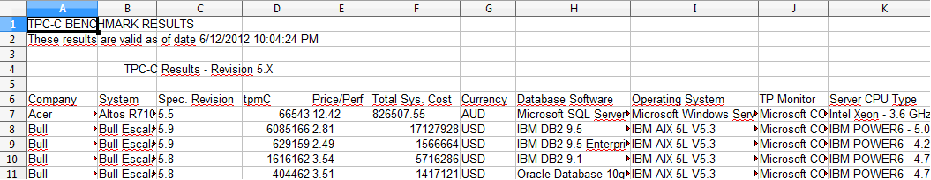
\includegraphics[width=0.90\textwidth]{figures/tpc_raw.png}
\caption{A tisztítatlan adathalmaz importálás után \label{fig:tpc_raw}}
\end{figure}

A tisztítás lépései (csak hogy lássák, hogy mik a fontosabb lépések):
\begin{sajat_itemize}
\item importálás táblázatkezelőbe
\item felesleges sorok eltávolítása
\item felesleges oszlopok eltávolítása (itt pl. spec. revision, withdraw stb.)
\item tizedespont vs. vessző átalakítások a számokat tartalmazó cellákban
\item új származtatott oszlopok felvétele (itt pl. Price/Perf (USD) és Total Sys. Cost (USD))
\item adatok aggregálása (itt pl. Database Software, Operating System)
\item exportálás (esetünkben tabulált értékek, hogy a később bemutatásra kerülő Mondriánba tudjuk importálni)
\end{sajat_itemize}

%------------------------------------------------------------------------------
\section{Feladatok}

\subsection{Mely években megjelent konfigurációkat tartalmazza a benchmark? Mennyire használható/releváns napjainkban?}
\subsubsection*{Megoldás}
Válasszuk ki az \texttt{Availability\_Date\_year} oszlopot, majd Plot $\rightarrow$ Barchart. Látható, hogy 2009-től megfogyatkozott a feltöltött eredmények száma.

\subsection{Az egyes beszállítók mely években voltak aktívak? Mely beszállító a nagy játékos?}
\subsubsection*{Megoldás}
Válasszuk ki a \texttt{Company} oszlopot, majd Plot $\rightarrow$ Barchart. Az egyes beszállítók neveire kattintva az éveket tartalmazó ablakban láthatjuk az aktív éveket.
\subsubsection*{Megállapítások, megjegyzések}
A HP minden évben adott ki konfigurációt (kivétel 2012, de még nincs vége az évnek), az Oracle csak az utóbbi két évben.

\subsection{Ha cégünk igényeit egy alacsonyabb teljesítményű konfigurációval is ki tudjuk elégíteni, akkor mely beszállítók közül válasszunk?}
\subsubsection*{Megoldás}
Nézzük meg a tpmC eloszlását. Ehhez válasszuk ki a \texttt{tpmC} oszlopot, majd Plot $\rightarrow$ Histogram. A bal szélső oszlopra kattintva a Company nézetén láthatjuk a szóba jöhető beszállítókat. A hisztogram bin szélességét a \textit{Ctrl + UP/DOWN} billentyűkkel módosíthatjuk.
\subsubsection*{Megállapítások, megjegyzések}
A jobb szélső oszlop az Oracle csúcskategóriás klasztere.

\subsection{Mit lehet megállapítani a teljesítmény változásáról?}
\subsubsection*{Megoldás}
Válasszuk ki az \texttt{Availability\_Date\_year} vagy \texttt{Availability\_Date\_day}, majd a \texttt{tpmC} oszlopokat, Plot $\rightarrow$ Scatterplot.
\subsubsection*{Megállapítások, megjegyzések}
Látható a teljesítmény növekedése, de néhány csúcsteljesítményű szerver kivételével inkább az alsó sávban helyezkednek el. Illesszünk regressziós görbét a pontokra. Az \texttt{Availability\_Date\_year - tpmC} scatterplotra jobb gombbal kattintva smoothers $\rightarrow$ ls-line. 

\todo{RServe hiánya esetén csak ez megy}

\todo{Többi simítógörbét megmutatni}

Ha valamelyik pont fölé visszük a kurzort és közben nyomva tartjuk a Ctrl-t akkor kiírja a ponthoz tartozó értékeket.
\subsubsection*{Ugyanez Boxplot alkalmazásával}
Válasszuk ki az \texttt{Availability\_Date\_year}, majd a \texttt{tpmC} oszlopokat, Plot $\rightarrow$ Boxplot y by x. Megfigyelhető a mediánok értékének növekedése.

\subsection{Hogyan alakulnak a tranzakciós és összköltségek?}
\subsubsection*{Megoldás}
Válasszuk ki az \texttt{Availability\_Date\_year}, majd a \texttt{Price\_per\_Perf\_in\_USD} oszlopokat, Plot $\rightarrow$ Scatterplot. Ezután az \texttt{Availability\_Date\_year}, \texttt{Total\_Sys\_Cost\_in\_USD} párost hasonló módon. Tegyünk regressziós görbét az ábrákra!
\todo{Leírni, hogyan tegyük oda a görbét!}
Láthatjuk, hogy a tranzakciós költségek csökkennek, viszont a teljes költségek inkább növekednek.
\subsubsection*{Megállapítások, megjegyzések}
Ha a tpmC ábrán kijelöljük a felső néhány pontot, akkor megállapíthatjuk, hogy a teljes költségek ugyan magasak, de a teljesítmény/ár arány még mindig jónak számít.

\subsection{Milyen adatbázis-kezelő szoftvert válasszunk, ha még mindig az olcsóbb megoldást szeretnénk használni?}
\subsubsection*{Megoldás}
Válasszuk ki a \texttt{Database\_Software} oszlopot, majd Plot $\rightarrow$ Barchart. A teljes költséget ábrázoló ploton jelöljük ki az alsó pontokat.
\subsubsection*{Megállapítások, megjegyzések}
Jól látható, hogy az MS SQL-es konfigurációk inkább az alsó és középső árkategóriákat fedik le, míg a felső kategória az Oracle-re és IBM-re jellemző.

\subsection{Milyen operációs rendszert válasszunk, ha a teljes költséget minimalizálni akarjuk?}
\subsubsection*{Megoldás}
Az \texttt{Operating\_System} oszlopból készítsünk egy barchartot, majd az \texttt{Availability\_Date\_year} - \texttt{Total\_Sys\_Cost\_in\_USD} scatterploton jelöljük ki az alsó pontokat. Látható, hogy főleg az MS Windows-os és Oracle Enterprise Linux-os konfigurációk a legolcsóbbak a teljes költséget nézve.
\subsubsection*{Megállapítások, megjegyzések}
Az \texttt{Availability\_Date\_year} - \texttt{tpmC} scatterploton kijelölve a felső pontokat látható, hogy a legnagyobb teljesítményt nyújtó gépeken Unix/Linux variánsok futnak, míg az \texttt{Operating\_System} barcharton a Windows-ra kattintva láthatjuk a tpmC ábráján, hogy ezen konfigurációk teljesítménye nem a legjobb.

\subsection{Melyik beszállító melyik adatbázis-kezelőben és operációs rendszerben ,,utazik''?}
\subsubsection*{Megoldás}
A már meglévő \texttt{Operating\_System}, \texttt{Database\_Software} és \texttt{Company} barchartok esetén a beszállítókat végig kattintgatva megvizsgálhatjuk, hogy mely OS-eket és DBMS-eket preferálják.

\subsection{Melyik beszállítót, adatbázis-kezelőt és operációs rendszert tartalmazza a leggyakrabban az adathalmaz?}
\subsubsection*{Megoldás}
Vegyünk fel mozaik diagramokat! Ehhez válasszuk ki a \texttt{Company} és \texttt{Database\_Software} oszlopokat, ezután Plot $\rightarrow$ Mosaic Plot, majd végezzük el ugyanezt a \texttt{Company} és \texttt{Operating\_System} oszlopokra is. A legnagyobb területű téglalapokat ki választva nézhetjük meg, hogy melyik a legelterjedtebb OS, DBMS és beszállító a piacon.
\subsubsection*{Megállapítások, megjegyzések}
A legnagyobb téglalapot a HP - MS Windows - MS SQL hármas birtokolja, ami természetesen valószínűleg nem független az elterjedtségtől sem.

\subsection{Próbáljunk összefüggést találni a teljesítmények, költségek, operációs rendszerek és adatbázis-kezelők között!}
\subsubsection*{Megoldás}
Jelöljük ki a \texttt{Company}, \texttt{tpmC}, \texttt{Price\_per\_Perf\_in\_USD}, \texttt{Total\_Sys\_Cost\_in\_USD}, \\ \texttt{Database\_Software},  \texttt{Operating\_System} és \texttt{Currency} oszlopokat, majd Plot $\rightarrow$ Parallel Coordinates.
\subsubsection*{Megállapítások, megjegyzések}
Az MSSQL fajlagosan (tmpC/USD) drága, de az összköltségük ezeknek a konfigurációknak alacsony. A Windows alapú rendszerek olcsóbbak, de rosszabb teljesítményt is nyújtanak. Az AIX operációs rendszerre csak DB2, Oracle és hatékonynak mondható adatbázis-kezelők vannak.
A párhuzamos koordináták módszere arra is alkalmas, hogy szelektáljunk a változók között. Pl. a Currency oszlopnál látszik, hogy semmihez nincs köze. Fontos a változók sorrendje (pl. \texttt{Database\_Software}, \texttt{Operating\_System} egymás mellé érdemes helyezni).

\end{document}